\section{Software arkitektur}

\subsection{Fokuspunkter}

\begin{itemize}
	\item Redegøre for begrebet softwarearkitektur.
	\item Giv et eksempel på en typisk softwarearkitektur og dens anvendelse?
	\item Hvordan udarbejdes en software arkitektur?
	\item Hvordan dokumenteres en software arkitektur?
\end{itemize}

\subsection{Redegør for begrebet softwarearkitektur}
\textit{''The highest-level breakdown of a system into its parts; the decisions that are hard to change; ...  and, in the end, architecture boils down to whatever the important stuff is.''}

\subsubsection{Hvad er en software arkitektur?}
Den højeste abstraktion.

\begin{itemize}
	\item Fokuserer på de større elementer og komponenter.
	\begin{itemize}
		\item Hvordan er de organiserede.
		\item Hvordan interagerer de?
		\item Er der nogle problematiske områder? (Areas of concern).\todo{nøjagtig formulering?}
	\end{itemize}
	\item Software Design er en realisering af arkitekturen bag.
	\item Arkitekturen viser de elemter som er svære at ændre.\todo{svære hvordan?}
	\item Viser også de elemter der er de vigtigste.
\end{itemize}

\subsubsection{Hvorfor er det vigtigt?}
Med komplekse systemer er det vigtigt at have et solidt fundament.

\begin{itemize}
	\item Der er følgende risici uden en arkitektur:
	\begin{itemize}
		\item Hovedscenarier kan overses.\todo{Defineres disse ikke FØR arkitekturen?}
		\item Almindelige problemer bliver overset.\todo{igen, hvorfor?}
		\item At værdsætte fremtidige konsekvenser på baggrund af afgørende beslutninger.\todo{føles som øregas}
	\end{itemize}
\end{itemize}

\subsubsection{Generelle overvejselser}
\begin{itemize}
	\item \textbf{Applikationstype} - Mobile app, web app osv.
	\item \textbf{Deployment strategi} - Distribueret/ikke distribueret, runtime kørsel, mnætværksinfrastruktur.
	\item \textbf{Teknologier} - Protokoller, Sprog, etc - Hvilke skal i bruges?
	\item \textbf{Quality attributter} - Kvalitet af systemet.
	\begin{itemize}
		\item Conceptual integrity.\todo{what is?}
		\item Maintainablity.
		\item Reusability.
		\item Performance.
		\item Security.
		\item Scalability.
		\item Reliability.
	\end{itemize}
	\item \textbf{Design kvalitet}
	\begin{itemize}
		\item Supportability.
		\item Testability.
	\end{itemize}
\end{itemize}

\subsubsection{Architectural Styles}
En arkitektur stil definerer en familie af systemer med ens struktur, navne af komponenter og connectors og med restriktioner omkring hvordan disse kan forbindes. De blandes ofte (på sammen måde som design patterns) - der bruges næsten aldrig kun een style.

\paragraph{Typer af styles (almindelige)}

\todo{savner forklaring af nogle de nedstående...}
\begin{itemize}
	\item Client/Server.
	\item Component based.
	\item Domain Driven Design.
	\item Layered.
	\item Message bus.
	\item N-tier/3-Tier.
	\item Object Oriented.
	\item Service oriented.
\end{itemize}


\subsection{Giv et eksempel på en typisk softwarearkitektur og dens anvendelse}

\subsubsection{Layer}
\begin{itemize}
	\item Et layer er en grovkornet gruppering af: \textit{klasser, packages, og subsystemer}.
	\item Sørger for koblingsgraden i et system.\todo{hvordan ''sørger'' den for det?}
	\item Organisering af lag:
	\begin{itemize}
		\item Højere lag kalder funktioner i lavere lag.
		\item Lavere lag må ikke kalde på funktioner i højere lag. Lavere lag må dog godt notificere højere lag omkring hendelser med f.eks. observer pattern eller call-back funktions pointere (events).
	\end{itemize}
	\item Layer vs Tier - Layer er en \textbf{logisk separering}, hvorimod Tier er en repræsentation af den \textbf{fysiske seaparering}.
\end{itemize}

\paragraph{Fordele ved Layer}
\begin{itemize}
	\item Separation af ansvar (SRP).
	\begin{itemize}
		\item Separation af applikationsspecifik logik fra generel logik.
		\item Separation af høj niveau fra lav-niveau logik.
	\end{itemize}
	\item Reducerer kobling og afhængigheder.
	\item Større samhørighed.
	\item Højt potentiale for genbrug.
	\item Forholdsvist let at forstå/gennemskue.
	\item \textbf{Fremmer parallel udviking} da systemet bliver delt op i logiske segmenter.
	\item Et lag kan udskriftes hvis der er brugt interface baseret programmering.
\end{itemize}

\paragraph{Eksempel på layers}
Figur~\ref{fig:guiblldab} viser hvordan en layeropdelt arkitektur kunne se ud for et system som skal have en GUI og Database med et Business Logik niveau imellem.

\begin{figure}[h]
	\centering
	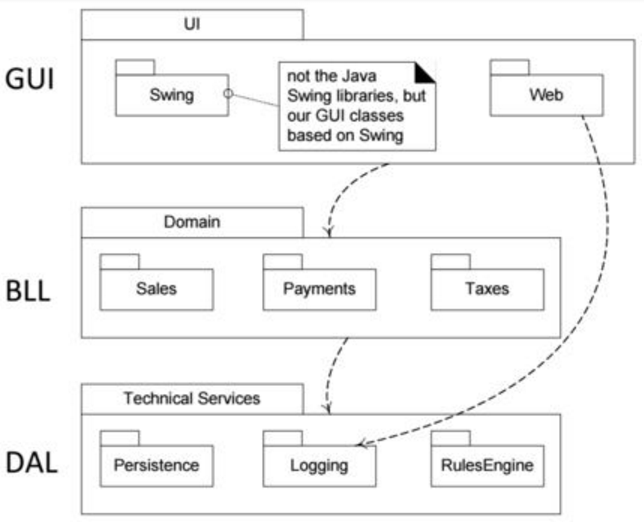
\includegraphics[width=0.7\linewidth]{figs/guiblldal}
	\caption{Arkitektur for et system med GUI, BLL og DAB logik.}
	\label{fig:guiblldab}
\end{figure}

Ligeledes kan man på figur~\ref{fig:osimodel} se den samme lagdeling i netværks modellen OSI\footnote{OSI: Open Systems Interconnection.}, som viser hvordan lagene imellem bruger hinanden.

\begin{figure}[h]
	\centering
	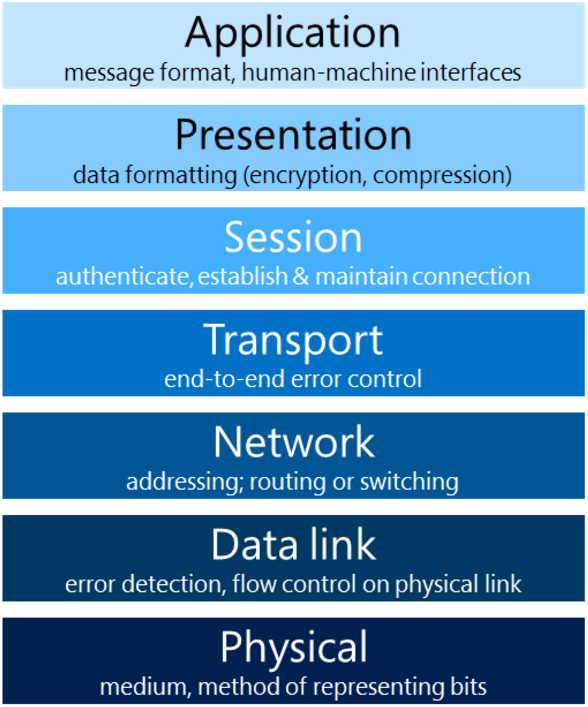
\includegraphics[width=0.5\linewidth]{figs/osimodel}
	\caption{Netværksarkitektur, Open Systems Interconnection Model (OSI model).}
	\label{fig:osimodel}
\end{figure}

\subsection{Hvordan udarbejdes en software arkitektur}
Der findes flere værktøjer:

\begin{itemize}
	\item ROPES: \textbf{R}apid \textbf{O}bject-oriented \textbf{P}rocess for \textbf{E}mbedded \textbf{S}ystems.\\
	Som navnet antyder er det primært til embedded software.
	\begin{itemize}
		\item Har 3 faser:
		\begin{itemize}
			\item Architectural.
			\item Mechanistic.
			\item Detailed Design (implementation).
		\end{itemize}
	\end{itemize}
	\item Iterativ (den vi mest bruger)
	\begin{itemize}
		\item 5 punkter, hvor de sidste 4 gentages iterativt, illustreret i figur~\ref{fig:arc_ite} og videre beskrevet i afsnit~\ref{sec:arc_ite}.
		\begin{enumerate}
			\item Identify architecture objectives.
			\item Identify key scenarios.
			\item Create application overview.
			\item Identify key issues.
			\item Define candidate solutions.
		\end{enumerate}
	\end{itemize}
\end{itemize}

\begin{figure}[h]
	\centering
	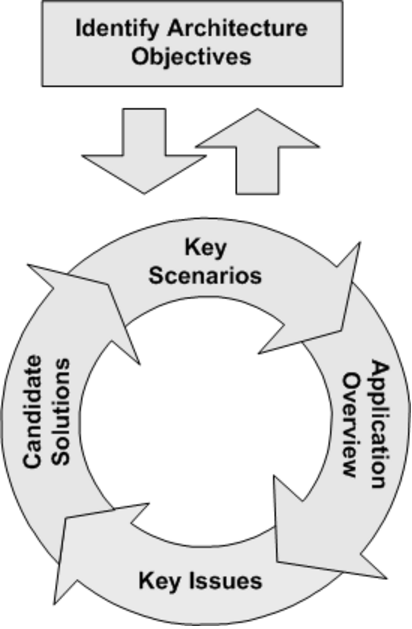
\includegraphics[width=0.5\linewidth]{figs/arc_ite}
	\caption{Process for iterativ arkitekturudvikling.}
	\label{fig:arc_ite}
\end{figure}

\subsubsection{Brug af Iterativ process}\label{sec:arc_ite}
Følgende trin anvendes i udvikling af produkt med iterativ projekt.

\paragraph{Identify Architecture Objectives}
\begin{itemize}
	\item Klare mål hjælper med at fokusere på arkitekturen og løse de konkrete probelmer i designet.
	\item Identificer arkitektur
\end{itemize}

\paragraph{Identify Key Scenarios}

\paragraph{Create Application Overview}

\paragraph{Identify Key Issues}

\paragraph{Define Candidate Solutions}

\subsection{Hvordan dokumenteres en software arkitektur}